\section{PRELIMINARIES AND BACKGROUND}
\label{pre}

In this section, we provide background information about the stream data processing engines and their features used in this paper. We analyze Apache Storm, Apache Spark, and Apache Flink as they are the most mature and accepted ones in both academia and  industry.
% and community driven stream data processing engines.  

\subsection{Apache Storm}

Apache Storm is a distributed stream processing framework, which was open sourced after being acquired by Twitter \cite{storm}. %todo[inline]{here we need a citation or link or both -> fixed}
Storm operates on tuple streams and provides record-by-record stream processing. It supports an at-least-once processing  semantics and guarantees all tuples to be processed. In failure cases, events are replayed. Storm also supports exactly-once processing semantics with its Trident abstraction \cite{trident}. %\todo[inline]{citation or link or both -> fixed} 
Stream processing programs are represented by a computational topology, which consists of spouts and bolts. Spouts are source operators and bolts are processing and sink operators. A Storm topology forms a directed acyclic graph (DAG), where the edges are tuple streams and vertices are operators (bolts and spouts). When a spout or bolt emits a tuple, the bolts that are subscribed to this spout or bolt receive input. 

Storm's lower level APIs provide little support for automatic memory and state management. Therefore, choosing the right data structure for state management and utilizing memory efficiently by making computations incrementally  is up to the user. Storm supports caching and batching the state transition. However, the efficiency of a particular operation degrades as the size of the state grows. 

 \todo[inline]{AK: what is the "state transition" mentioned above?}

Storm has built-in support for windowing.  Although the information of expired, newly arrived, and total tuples within a window is provided through APIs, the incremental state management is not transparent to the users. Trident, on the other hand,  has built-in support for partitioned windowed joins and aggregations. Storm supports sliding and tumbling windows on processing time and event time. For event-time windows, tuples need to have a dedicated timestamp field so that the engine can create periodic watermarks.  Any worker process in Storm topology sends acknowledgements to the source executor for a processed tuple. In case of failure Storm sends the messages again. One of the downsides of Storm's use of acknowledgments is that the tuples can be only be acknowledged once a window operator  completely flushes them out of a window. This can be an issue on windows with large length and small slide.%\todo[inline]{when did you explain the acknowledgements? => fixed}

Backpressure is one of the key features of SDPSs. It refers to the situation where a system is receiving data at a higher rate than it can process. For example, this can occur during temporary load spikes. Storm supports backpressure although the feature is not mature yet \cite{WinNT}. This was confirmed throughout our experiments as well. %\todo[inline]{Maybe explain backpressure in general first => fixed} 
Storm uses an extra backpressure thread inside the system. Once the receiver queue of an operator is full, the backpressure thread is notified. %\todo[inline]{Where does Zookeeper come from now? If it is essential, you should introduce it with citation first. Otherwise, do not talk about Zookeeper, since you are not discussing the internal architecture of the systems anyway.=> fixed} 
This way Storm can notify all workers that the system is overloaded. Due to its high complexity, Storm's backpressure feature can stall the system and, therefore, it is not enabled by default in the current version.


\subsection{Apache Spark}
Apache Spark is an open source big data processing engine, originally developed at the University of California, Berkeley \cite{spark}. %\todo[inline]{Missing link or citation or both=>fixed}
Unlike Storm and Flink, which support one record at a time, Spark Streaming inherits its architecture from batch processing, which supports processing records in micro-batches. Throughout this paper, we refer to Spark Streaming as simply Spark. The Resilient Distributed Dataset (RDD) is a fault-tolerant abstraction of Spark, which enables in-memory, parallel computation in  distributed cluster environments \cite{zaharia2012resilient}.  


%\begin{figure}[h]
%\centering
%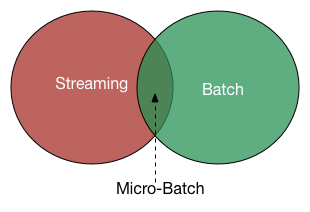
\includegraphics[width=0.5\textwidth]{eps/streambatch}
%\caption{Conceptual view of micro-batching}
%\label{fig_micro_batch}
%\end{figure}


One of Spark's features is its support of lazy evaluation. This enables the engine to run more efficiently. 
\todo[inline]{AK: why does lazy evaluatin run efficiently? CAreful waht you state in general. I would remove the above sentence without the paper suffering from its absense.}

Spark  supports stage-oriented scheduling. Initially, it computes a DAG  of stages for each submitted job.  Then it keeps track of materialized  RDDs and outputs from each  stage, and finally finds a minimal schedule. 

Unlike Flink and Storm, which also work based on DAG execution graphs, Spark's computing unit in a graph (edge) is a data set rather than streaming records and each vertex in a graph is a stage rather than individual operators. RDDs are guaranteed to be processed in order in a single DStream (Discretized Stream), which  is a continuous sequence of RDDs. However, there is no guaranteed ordering within RDDs  since each RDD is processed in parallel. 

Spark has improved its memory management significantly in the recent releases. The system shares the memory  between execution and storage. This unified memory management supports dynamic memory management between the two modules. Moreover, Spark supports dynamic memory management throughout the tasks and within operators of each task. 

Spark has a built-in support for windowed calculations. It supports only windows defined by processing time. The window size must be a multiple of the batch interval, because a window keeps a particular number of batches until it is purged. Choosing the  batch interval can heavily affect the performance of window-based analytics. First, the latency and response time of windowed analytics is strongly relying on the batch interval. Second, supporting only processing time windowed analytics, can be a severe limitation for some use-cases.


Spark also supports backpressure. It handles backpressure by putting a bound to the block size. Depending on the duration and load of each mini-batch job, the effectiveness of backpressure signal handling from source to destination may vary. 
%todo[inline]{fast enough for what?=>fixed}

\subsection{Apache Flink}
Apache Flink started off as an open source big data processing system at TU Berlin, leveraging in major parts the codebase of the Stratosphere project [9].
\todo[inline]{Fix citation, add citation to the new flink paper as well as stratospherein the respective places.}

At its core, Flink is a distributed dataflow engine. Like in Storm, a Flink runtime program is a DAG of operators connected with data streams. Flink's runtime engine supports unified processing of batch (bounded) and stream (unbounded) data, considering former as being the special case of the latter.

Flink provides its own memory management to avoid long running JVM's garbage collector stalls by serializing data into memory segments. 
The data exchange in distributed environments is achieved via buffers. A producer takes a buffer from the pool, fills it up with data, then the consumer receives the data and frees the buffer informing the memory manager. Flink provides a wide range of high level and user friendly APIs to manage  state.  Incremental state update, managing the memory, or checkpointing with big states are performed automatically and transparently to user. 

Flink has a strong feature set for building and evaluating windows on data streams. With a wide range of pre-defined windowing operators, it supports user-defined windows with custom logic. The engine provides processing-time, event-time, and ingestion-time semantics. When using processing time, like Spark, windows are defined with respect to the wall clock of the machine that is responsible for building and processing  a window. When using event time, on the other hand, the notion of time is determined by the timestamp attached to an event, which typically resembles its creation time. Like in Storm, the timestamps must be attached to each event record as a separate field. At ingestion time, the system processes records with event time semantics on these timestamps. Flink has support for out-of-ordered streams, which were motivated from Googles MilWheel and Dataflow papers \cite{akidau2013millwheel,akidau2015dataflow}. Flink also supports backpressure. It uses blocking queues. Once the congestion is detected this information is automatically transferred to upstream operators at negligible cost. 

